\let\negmedspace\undefined
\let\negthickspace\undefined
\documentclass[journal]{IEEEtran}
\usepackage[a5paper, margin=10mm, onecolumn]{geometry}
%\usepackage{lmodern} % Ensure lmodern is loaded for pdflatex
\usepackage{tfrupee} % Include tfrupee package

\setlength{\headheight}{1cm} % Set the height of the header box
\setlength{\headsep}{0mm}     % Set the distance between the header box and the top of the text

\usepackage{gvv-book}
\usepackage{gvv}
\usepackage{cite}
\usepackage{amsmath,amssymb,amsfonts,amsthm}
\usepackage{algorithmic}
\usepackage{graphicx}
\usepackage{textcomp}
\usepackage{xcolor}
\usepackage{txfonts}
\usepackage{listings}
\usepackage{enumitem}
\usepackage{mathtools}
\usepackage{gensymb}
\usepackage{comment}
\usepackage[breaklinks=true]{hyperref}
\usepackage{tkz-euclide} 
\usepackage{listings}
% \usepackage{gvv}                                        
\def\inputGnumericTable{}                                 
\usepackage[latin1]{inputenc}                                
\usepackage{color}                                            
\usepackage{array}                                            
\usepackage{longtable}                                       
\usepackage{calc}                                             
\usepackage{multirow}                                         
\usepackage{hhline}                                           
\usepackage{ifthen}                                           
\usepackage{lscape}
\begin{document}

\bibliographystyle{IEEEtran}
\vspace{3cm}

\title{NCERT-11.16.3.13.1}
\author{EE24BTECH11023 - RASAGNA}
% \maketitle
% \newpage
% \bigskip
{\let\newpage\relax\maketitle}
\renewcommand{\thefigure}{\theenumi}
\renewcommand{\thetable}{\theenumi}
\setlength{\intextsep}{10pt} % Space between text and floats
\numberwithin{equation}{enumi}
\numberwithin{figure}{enumi}
\renewcommand{\thetable}{\theenumi}
\textbf{Question:}
Given:\\
\begin{align}
Pr{\brak{A}}=\frac{1}{3}\\
Pr{\brak{B}}=\frac{1}{5}\\
Pr{\brak{AB}}=\frac{1}{15}
\end{align}
Then find the value of $P{\brak{A+B}}$.\\
\textbf{Theoritical Solution:}\\
Let $A$ and $B$ be two sets ;
\begin{align}
    A=AB^{'}+AB\\
    B=A^{'}B+AB
\end{align}
Adding the equations $\brak{0.4}$ and $\brak{0.5}$ we get;
\begin{align}
    A+B=A^{'}B+AB^{'}+AB
\end{align}
Here $A^{'}B,AB^{'},AB$ are disjoint.
\begin{align}
    \therefore Pr(A+B)=Pr(A)+Pr(B)-Pr(AB)
\end{align}
Substituting the values of $Pr(A),Pr(B)$ and $Pr(A \cap B)$ in the equation $\brak{0.7}$ we get the value of $Pr(A+B)$ as,
\begin{align}
    Pr(A+B)=\frac{1}{3}+\frac{1}{5}-\frac{1}{15}
\end{align}
\begin{align}
    \therefore Pr(A + B)=\frac{7}{15}
\end{align}
\textbf{Computational Solution}\\
Let $X,Y,Z$ be an indicator random variables of the event $A,B,AB$.\\
Where $X,Y,Z$ are defined as:
\begin{align}
	X =
	\begin{cases}
		1 &; A\\
		0 &; A^{'}\\
	\end{cases}
\end{align}
\begin{align}
	Y =
	\begin{cases}
		1 &; B\\
		0 &; B^{'}\\
	\end{cases}
\end{align}
\begin{align}
	Z =
	\begin{cases}
		1 &; AB\\
		0 &; \brak{AB}^{'}\\
	\end{cases}
\end{align}
The PMF of the random variables $X,Y,Z$ are:
\begin{align}
	p_{X}\brak{n} =
	\begin{cases}
		p_1 &; n = 1\\
		1 - p_1 &; n = 0
	\end{cases}
\end{align}
\begin{align}
	p_{Y}\brak{n} =
	\begin{cases}
		p_2 & ;n = 1\\
		1 - p_2 &; n = 0
	\end{cases}
\end{align}
\begin{align}
	p_{Z}\brak{n} =
	\begin{cases}
		p_3 &; n = 1\\
		1 - p_3 &; n = 0
	\end{cases}
\end{align}
Here,
\begin{align}
	p_1 &= \frac{1}{3}\\
	p_2 &= \frac{1}{5}\\
	p_3 &= \frac{1}{15}
\end{align}
Now let us define another random variable K.\\
Where,
\begin{align}
	K = X + Y - Z
\end{align}
$Z$ can never be $0$ whenever $X$ and $Y$ are $1$ (Because (1).(1) is never equal to 0).\\
So, $K$ is also an Indicator Random variable.\\
Its PMF is defined as:
\begin{align}
	p_{K}\brak{n} =
	\begin{cases}
		p &; n = 1\\
		1 - p &; n = 0
	\end{cases}
\end{align}
From $\brak{0.20}$,
\begin{align}
	E\brak{K} &= E\brak{X + Y - Z}\\
	E\brak{K} &= E\brak{X} + E\brak{Y} - E\brak{Z}\\
	1.\brak{p} + 0.\brak{1 - p} &= 1.\brak{p_1} + 0.\brak{1 - p_1} + 1.\brak{p_2} + 0.\brak{1 - p_2} - 1.\brak{p_3} - 0.\brak{1 - p_3}\\
	p &= p_1 + p_2 - p_3
\end{align}
Here
\begin{align}
	\Pr\brak{A} = p_1\\
	\Pr\brak{B} = p_2\\
	\Pr\brak{AB} = p_3
\end{align}
Therefore, from the axiom and equation \brak{0.25}\\
\begin{align}
	\Pr\brak{A + B} = \Pr\brak{A} + \Pr\brak{B} - \Pr\brak{AB}
\end{align}
\begin{align}
	p &= \Pr\brak{A + B}\\
	\Pr\brak{A + B} &= \frac{1}{3} + \frac{1}{5} - \frac{1}{15}\\
	\therefore \Pr\brak{A + B} &= \frac{7}{15}
\end{align}
\newpage
Here is the graph (Stem plot) of probabilities $Pr(A),Pr(B),Pr(AB)$ and $Pr(A+B)$\\
Blue colour represents theoritical values of the probabilities.\\
Brown colour represents Computed values of the probabilities.\\
\begin{figure}[h!]
	\centering
	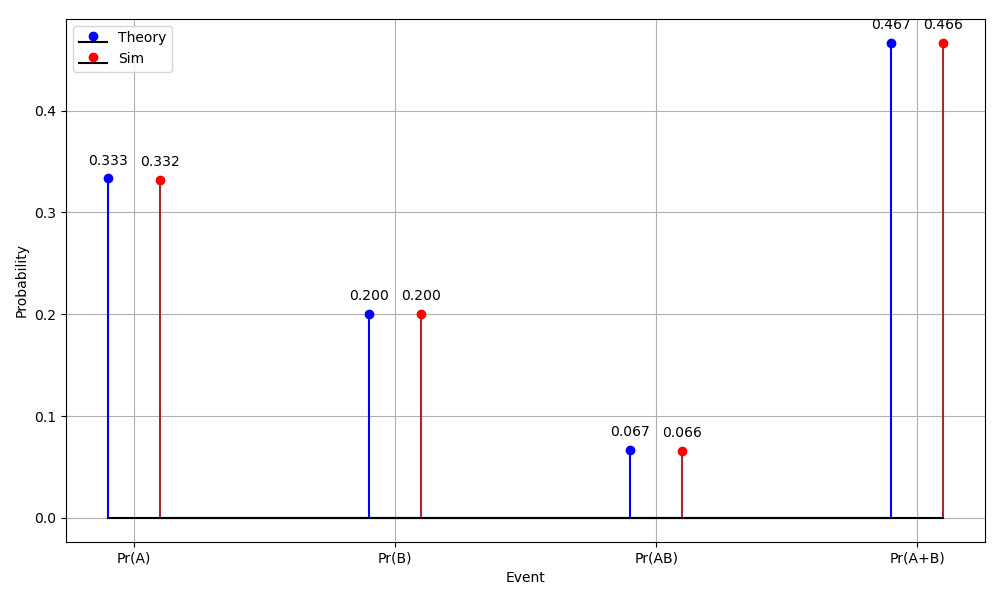
\includegraphics[width=1\columnwidth]{figs/prob.png}
\end{figure}
\end{document}